
Bộ Half Adder là khối cơ bản để xây dựng cho các mạch cộng phức tạp hơn như Full Adder và Multiple-bit Adder. Bộ Half Adder thực hiện phép cộng nhị phân của hai đầu vào 1-bit A và B, và đầu ra là SUM(S) và CARRY(C). Với $\text{SUM(S)} = A \oplus B$ và $\text{CARRY(C)} = A \& B$.
\begin{figure}[H]
	\centering
	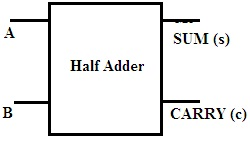
\includegraphics[width=0.5\linewidth]{./image/Half-Adder-blockblock.jpg}
	\caption{Bộ Half Adder}
	\label{f_block haft adder}
\end{figure}

Ta có bảng sự thật của mạch:

\begin{table}[H]
	\centering
	\begin{tabular}{|c|c|c|c|}
		\hline
		\multicolumn{2}{|c|}{Input} & \multicolumn{2}{c|}{Output} \\
		\hline
		A & B & SUM(S) & CARRY(C) \\
		\hline
		0 & 0 & 0 & 0 \\
		\hline
		0 & 1 & 1 & 0 \\
		\hline
		1 & 0 & 1 & 0 \\
		\hline
		1 & 1 & 0 & 1 \\
		\hline
	\end{tabular}
	\caption{Bảng sự thật của bộ Half Adder}
	\label{t_true table}
\end{table}

Thực hiện bộ Half Adder:
\begin{itemize}[label = -]
	\item Bộ Half Adder thực hiện bảng cổng XOR và cổng AND:
	\begin{figure}[H]
		\centering
		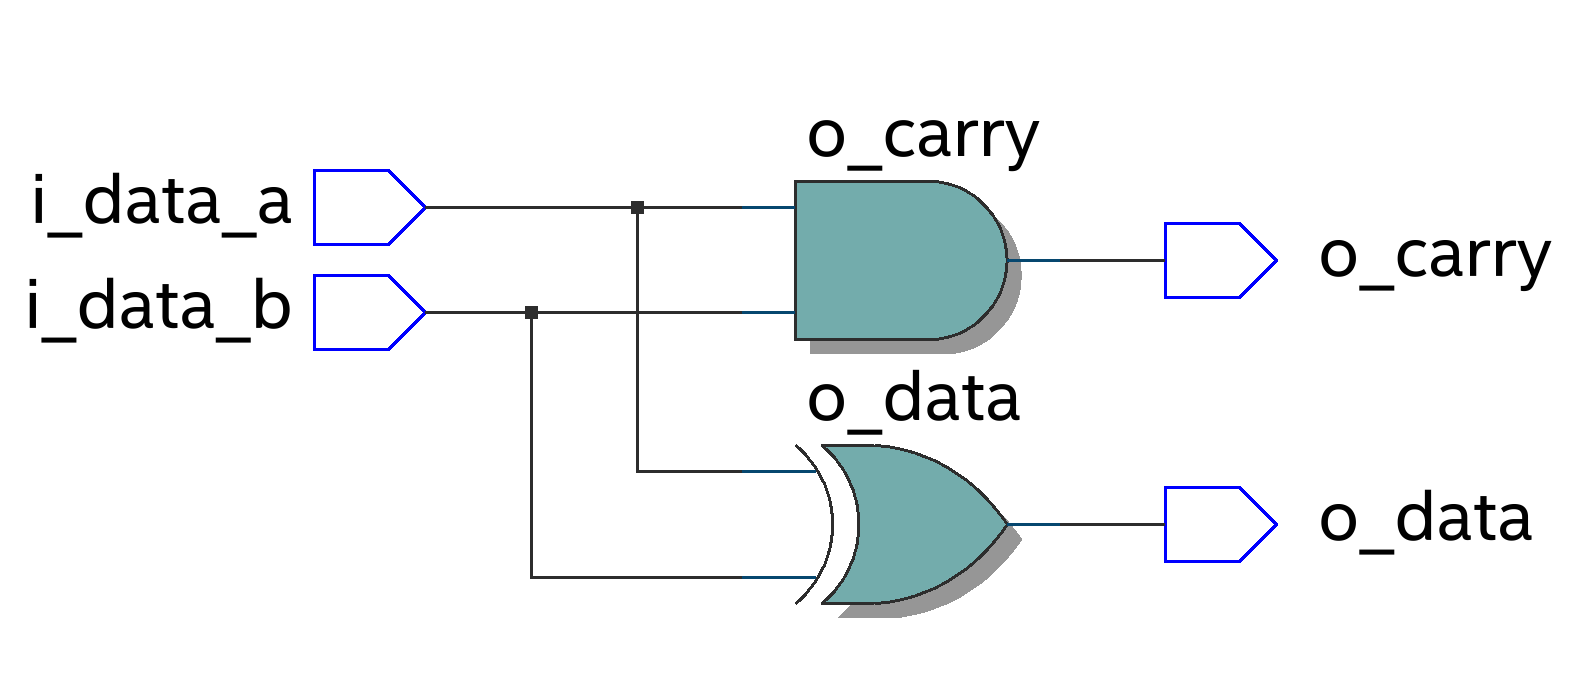
\includegraphics[width = 0.5\linewidth]{./image/half_adder_xor_and.png}
		\caption{Bộ Half Adder thực hiện bẳng cổng XOR và cổng AND}
		\label{f_half adder with xor and and}
	\end{figure}
	
	\lstinputlisting[style = SystemVerilog, caption = {Bộ Half Adder thực hiện bằng cổng XOR và cổng AND}]{./code/half_adder/half_adder_with_xor_and.sv}
	\item Bộ Half Adder thực hiện bẳng cổng NOR:
	\begin{figure}[H]
		\centering
		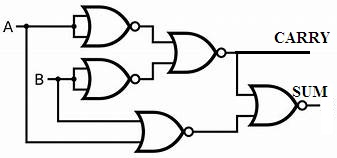
\includegraphics[width = .5\linewidth]{./image/Half-Adder-using-NOR-gates.jpg}
		\caption{Bộ Half Adder thực hiện bằng cổng NOR}
		\label{f_half adder with nor}
	\end{figure}
	
	\lstinputlisting[style=SystemVerilog, caption={Bộ Half Adder thực hiện bằng cổng NOR}]{./code/half_adder/half_adder_with_nor.sv}
	\item Bộ Half Adder thực hiện bằng cổng NAND:
	\begin{figure}[H]
		\centering
		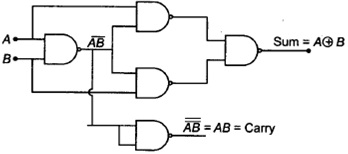
\includegraphics[width = 0.5\linewidth]{./image/Half-Adder-NAND-gates.jpg}
		\caption{Bộ Half Adder thực hiện bằng cổng NAND}
		\label{f_half adder with nand}
		
		\lstinputlisting[style=SystemVerilog, caption={Bộ Half Adder thực hiện bằng cổng NAND}]{./code/half_adder/half_adder_with_nand.sv}
	\end{figure}
\end{itemize}

Sử dụng test case sau đây để tiến hành kiểm tra lại hệ thống trên:
\begin{lstlisting}[style = C, caption={Test bench của bộ Half Adder}]
	int main(int argc, char **argv) {
		Verilated::commandArgs(argc, argv);
		
		VName_module* uut = new VName_module;
		
		// Test case
		printf("A B | Sum Carry\n");
		printf("-------------------\n");
		
		// case 1: A = 0, B = 0
		uut->i_data_a = 0; 
		uut->i_data_b = 0;
		uut->eval();
		printf("%d %d |  %d    %d\n", uut->i_data_a, uut->i_data_b, uut->o_data, uut->o_carry);
		
		// case 2: A = 0, B = 1
		uut->i_data_a = 0; 
		uut->i_data_b = 1;
		uut->eval();
		printf("%d %d |  %d    %d\n", uut->i_data_a, uut->i_data_b, uut->o_data, uut->o_carry);
		
		// case 3: A = 1, B = 0
		uut->i_data_a = 1; 
		uut->i_data_b = 0;
		uut->eval();
		printf("%d %d |  %d    %d\n", uut->i_data_a, uut->i_data_b, uut->o_data, uut->o_carry);
		
		// case 4: A = 1, B = 1
		uut->i_data_a = 1; 
		uut->i_data_b = 1;
		uut->eval();
		printf("%d %d |  %d    %d\n", uut->i_data_a, uut->i_data_b, uut->o_data, uut->o_carry);
		
		// deleted object
		delete uut;
		return 0;
	}
\end{lstlisting}

Kết quả:


	\begin{lstlisting}[style = C, caption={Sử dụng cổng XOR và cổng AND}]
		$ ./obj_dir/Vhalf_adder_with_xor_and 
		A B | Sum Carry
		-------------------
		0 0 |  0    0
		0 1 |  1    0
		1 0 |  1    0
		1 1 |  0    1
	\end{lstlisting}
	
	\begin{lstlisting}[style=C, caption={Sử dụng cổng NOR}]
		$ ./obj_dir/Vhalf_adder_with_nor 
		A B | Sum Carry
		-------------------
		0 0 |  0    0
		0 1 |  1    0
		1 0 |  1    0
		1 1 |  0    1
	\end{lstlisting}
	
	\begin{lstlisting}[style = C, caption={Sử dụng cổng NAND}]
		$ ./obj_dir/Vhalf_adder_with_nand
		A B | Sum Carry
		-------------------
		0 0 |  0    0
		0 1 |  1    0
		1 0 |  1    0
		1 1 |  0    1
	\end{lstlisting}